% Sample file for AES paper
\documentclass[fleqn]{jaes}

% Metadata Information
\jyear{2026}
\jmonth{August}
%\jvol{69}
%\jnum{3}

\usepackage{amsmath}\setlength{\mathindent}{10pt}
\usepackage{bm}
\usepackage{csquotes}
\usepackage{graphicx}
\usepackage{booktabs}
\usepackage[inline]{enumitem}
\usepackage{fancybox}
\usepackage{lipsum}
\usepackage{xcolor}

% This let's you display \num{} formated numbers in bold.
\sisetup{
text-series-to-math = true,
propagate-math-font = true
}

\usepackage[capitalise]{cleveref}
  \crefformat{section}{\textsc{Sec.~#2#1#3}}
  \Crefformat{section}{\textsc{Sec.~#2#1#3}}
  \crefformat{figure}{{Fig.~#2#1#3}}
  \Crefformat{figure}{{Fig.~#2#1#3}}
  \crefformat{table}{{Table~#2#1#3}}
  \Crefformat{table}{{Table~#2#1#3}}


\usepackage[automake,acronym]{glossaries-extra}
\setabbreviationstyle[acronym]{long-short}
% JAES has a list of acronyms that don't require expanding. Use this style for those.
\setabbreviationstyle[alwaysshort]{short-nolong}
\makeglossaries 
\newabbreviation{sip}{SIP}{Stereo Image Profile}
\newabbreviation[category=alwaysshort]{vr}{VR}{Virtual Reality}
\newabbreviation[category=alwaysshort]{ar}{AR}{Augmented Reality}
\newabbreviation{xr}{XR}{Extended Reality}
\newabbreviation{srm}{SRM}{Spatial Release from Masking}
\newabbreviation[category=alwaysshort]{mushra}{MUSHRA}{MUltiple Stimuli with Hidden Reference and Anchor}
\newabbreviation{hrir}{HRIR}{Head-Related Impulse Response}
\newabbreviation{hints}{HINTS}{Human-Centered Intelligent Realities}
\newabbreviation{asa}{ASA}{Auditory Scene Analysis}
\newabbreviation{msa}{MSA}{Musical Scene Analysis}
\newabbreviation{tts}{TTS}{Text-to-Speech}
\newabbreviation{dj}{DJ}{Disc Jockey}
\newabbreviation{dof}{DOF}{Degrees of freedom}
\newabbreviation{cv}{CV}{Critical value}
\newabbreviation{bth}{BTH}{Blekinge Institute of Technology}
\newabbreviation{mpeg}{MPEG}{Moving Picture Experts Group}
\newabbreviation{acm}{ACM}{Association of Computing Machinery}



%% Template specific, to remove
% \usepackage{draftwatermark}
% \SetWatermarkText{TEMPLATE}
% \SetWatermarkColor[gray]{0.9}
% \SetWatermarkScale{0.85}

% \usepackage[left]{lineno} % [switch] option for outside two-column not compatibal with JAES template
% \linenumbers

%\usepackage{citesort}
% Tested successfully with todonotes pkg
\usepackage[]{todonotes}
\newcommand{\mytodo}[1]{\todo[inline,color=blue!10]{Todo: #1}}

\begin{document}

% Title portion
\title{Perceptual Evaluation of Binaurally Panned Speech and Music Mixtures}

% Page heads {Authors}{Short title}
\markboth{Mitic et. al.}{Percept. Eval. Binaurally Panned Speech and Music Mixtures}

%Author Info.
\authorgroup{
\author{Richard Mitic\thanks{These authors contributed equally to this work},\textsuperscript{1}\orcidlink{0000-0003-3232-191X}}
\aesrole{Student Member}{876446}, % For AES members, provide current membership role (Member, Associate Member, Student Member, Honorary Member, Fellow, or Life Member) and AES membership number
AND \author{Majed Elwardy\raisebox{2pt}{$\ast$},\textsuperscript{2}\orcidlink{0000-0002-7550-5818}}
% \aesrole{Fellow}{43549}
\email{(richard.mitic@mdu.se)\quad\quad\quad\quad\quad\quad\quad\quad\quad\quad\quad\quad\quad\quad\quad\quad\quad (majed.elwardy@bth.se)}
AND \author{Veronica Sundstedt,\textsuperscript{2}\orcidlink{0000-0003-3639-9327}}
AND \author{Andreas Rossholm,\textsuperscript{3}\orcidlink{0009-0001-5678-038X}}\aesrole{Member}{291625}
AND \author{Yan Hu,\textsuperscript{2}\orcidlink{0000-0002-3283-2819}}
\email{(veronica.sundstedt@bth.se) \quad\quad\quad\quad\quad\quad (arossholm@spotify.com) \quad\quad\quad\quad\quad\quad\quad\quad\quad\quad (yan.hu@bth.se)}
\affil{\textsuperscript{1}School of Innovation, Design and Engineering, Mälardalen University, Västerås, Sweden \\
\textsuperscript{2}Department of Computer Science, Blekinge Institute of Technology, Karlskrona, Sweden \\
\textsuperscript{3}Media Quality Lab, Spotify AB, Stockholm, Sweden}
}

%Abstract
\abstract{%
Music streaming services have the opportunity to adapt the listening experience for each user. This can include the option of interspersing speech audio with music tracks, providing interesting information to the listener. It is also possible to mix speech audio with music, although there is a lack of research that studies the most effective ways to achieve a pleasant listening experience. This paper describes a subjective test in which volunteering participants were asked to rate the pleasantness of music mixed with relevant speech. The speech signal was panned binaurally between 45\textdegree~left and 45\textdegree~right, in 15\textdegree~ increments, and mixed with various music tracks at equal loudness, with the hypothesis that this would improve the pleasantness ratings compared to centrally panned speech. The results indicate that the centre is not always the optimum panning position and that participants had strong individual preferences. Future work should concentrate on controlling and expanding the audio stimuli, and investigating the reasons for participants' preferences. }

\maketitle

% Keywords, provide at least 3 keywords
\begin{keywords}
Music, Speech, Music Mixtures, Binaural Panning, User Study, Subjective Test, Perceptual Evaluation
\end{keywords}

%Head 1
\section{Introduction}
\label{sec:intro}
When mixing a speech recording with a music track, the accepted norm in industry is to reduce the volume of the music to make the speech intelligible. This paradigm is called \enquote{ducking}, and is so widespread that literature on the subject generally does not acknowledge that other mixing techniques are available~\cite{torcoliPreferredLevelsBackground2019,torcoliBackgroundDuckingProduce2019,venkateshArtificiallySynthesisingData2021,hagedornAudiobearbeitungMitAudacity2015}. In the radio and TV industries in particular, there has been research into optimal ducking parameters such as speech-to-background level differences, and speech timing~\cite{torcoliPreferredLevelsBackground2019}. 

Another option is to intersperse speech and music so that they never mask each other \cite{SpotifyDebutsNew2023}. Alternatively, in the realm of \gls{vr} or \gls{ar}, it is standard practice to adjust the physical location of sound sources to achieve perceptual separation~\cite{lugasiSpeechEnhancementUsing2020,hsuModelMatchingPrincipleApplied2023}.

Previous literature generally forms the problem as one of speech intelligibility, with any music being classified as a \enquote{background} or \enquote{ambient} sound~\cite{torcoliPreferredLevelsBackground2019,hsuModelMatchingPrincipleApplied2023,hakeIndividualDifferencesAuditory2025}. In this paper we posit that the inverse is also valid - music is the dominant and most desirable sound, whereas speech is an addition. The question then becomes how to mix the two in such a way that the listener's enjoyment of the music is minimally affected. Consider the use case of a radio \gls{dj} providing commentary (which is typically done at the transition or mixing point between two tracks) or exercise instructions set over music. In both cases, music is the dominant auditory content and the speech consists of short and sparse interjections. 

During the rise of music streaming services in recent years, personalized experiences have been identified as a strong factor in their adoption by consumers~\cite{barataMusicStreamingServices2021}. When personalization is mentioned, it generally refers to recommending tracks or playlists that a user might like. Since personalization of the music choice serves to improve a listener's experience, it logically follows that enjoyment of the music is paramount whereas any additional speech might be treated as secondary.

More recently, other personalization options have emerged, such as personalized user interfaces~\cite{AIPersonalizationRevolutionizing2024}. In parallel, high-quality text-to-speech services have become much more readily available, to the point where they can be used to generate personalized informational audio about the music~\cite{SpotifyDebutsNew2023}. 

Although these new technologies are already established and being put into production, the usual practice of ducking the music when speech is present remains. There is currently little research on other methods to mix music and speech acceptably and pleasantly. For example, it is known that mixing music or acoustic noise with speech results in a drop in intelligibility and perceived quality \textit{of the speech itself}~\cite{fichnaPerceptualEvaluationSimulated2022}, but further research is required to determine how to minimally affect the perceived quality of the \textit{music}.

This paper describes a perceptual evaluation designed to investigate how the panning position of speech audio mixed with music influences the perceived pleasantness of the mixture as a whole. Speech audio was binaurally panned between 45\textdegree~left and 45\textdegree~right in 15\textdegree~increments, and overlaid on various music tracks.

The remainder of the paper is organized as follows. \cref{sec:background} describes the relevant concepts for the study and presents related work. The experimental method is presented in \cref{sec:method}, and the results are analysed and discussed in \cref{sec:results_analysis}. Finally, the work is concluded, and future work is suggested in \cref{sec:conclusions}.

\section{Background and related work}
\label{sec:background}

% Put this back in if we use the SIP diagrams for anything
% \gls{sip} refers to a description of the stereo field in an audio recording. There are multiple types of \gls{sip}, some of which are summarized in~\cite{miticObjectiveComparisonPanning2025}, which recommends modifying the existing types to fit a specific task. One such \gls{sip} is \enquote{Panning Histogram}~\cite{gomezMusicSimilaritySystems2008}, which describes the likelihood that a stereo audio signal has energy at a given azimuth position (and optionally in a given frequency band). Notably, the \enquote{panning azimuth} is a dimensionless value that spans from left to right but does not necessarily indicate a precise angle of incidence.


Binaural panning is an advanced audio spatialization technique in which a monophonic signal is modelled as a point source at a specific angle from the listener's ears. It can be achieved by convolving the mono signal with the left and right \gls{hrir} recorded from binaural microphones. Headphones are typically required to hear the correct effects of binaural panning. It differs from amplitude panning, in which the amplitude of a signal is adjusted in the left and right channels to make the audio source appear to come from a different direction. Amplitude panning is common in music production, whereas binaural panning is typically used more in \gls{vr}, \gls{ar}, and \gls{xr}.

\gls{srm} is a well-studied phenomenon in which humans can perceive more detail in two sounds that come from different directions than if they come from the same direction. The associated research problem is \enquote{The cocktail party effect}, which refers to the problem of perceiving speech in the presence of other interfering noises~\cite{litovskySpatialReleaseMasking2012}. \gls{srm} can be exploited to improve the clarity of recorded voices and to create a deeper sense of immersion in the final mix~\cite{stewartEssentialRadioSkills2015}.

The clarity and intelligibility of speech when masked with another sound source have been major research topics for decades. One particular area of interest is speech in reverberant environments, with research dating back to the mid 20th century and continuing to this day~\cite{haasInfluenceSingleEcho1972,liDiscussionCorrelationClarity2023}. A second broad area of speech intelligibility research is related to the effects of interference noise. This can take the form of other speakers, environmental noise, artificial noise, and (more recently) music. For example,~\cite{torcoliPreferredLevelsBackground2019} investigates the ducking parameters necessary for clear speech in TV audio mixes, concluding firstly that music needs to be attenuated by 10~dB in order to make speech intelligible, and secondly that listeners have highly personal preferences. In the \gls{vr} space, music has also been used as an interfering source with the express intention of measuring or improving the intelligibility of speech~\cite{akeroyd2ndClarityEnhancement2023,fichnaPerceptualEvaluationSimulated2022}. Until recently the perceptual quality of \textit{music} that has been distorted or manipulated in a \gls{vr} or \gls{ar} setting has been historically neglected~\cite{madsenMusicHearingAids2014,benjaminEvaluatingAudioQuality2024,hakeIndividualDifferencesAuditory2025}. This perceptual evaluation aims to investigate how music and speech can be mixed in a suitable way, with the previously mentioned use cases in mind.

\section{Method}
\label{sec:method}

This experiment aims to explore the subjective evaluation of spatialized speech in music. Data were collected using rankings and questionnaires. The test procedure follows a \glsxtrshort{mushra}-like structure~\cite{itu-r-bs.1534-3MethodSubjectiveAssessment2023}.

\subsection{Setup}
The experiment was conducted in a controlled laboratory environment, free from external disturbances. During the experiment, participants were comfortably seated on a soft chair. A Mac laptop was used to display the experiment stimuli, which consisted of a graphical interface, as shown in \cref{fig:interface}. A pair of Sennheiser HD 650 headphones was used together with a Focusrite Scarlett Solo 3rd Gen, to allow each participant to modify the volume to a suitable setting, as permitted by~\cite{itu-r-bs.1534-3MethodSubjectiveAssessment2023}.

\begin{figure*}[h]
\centerline{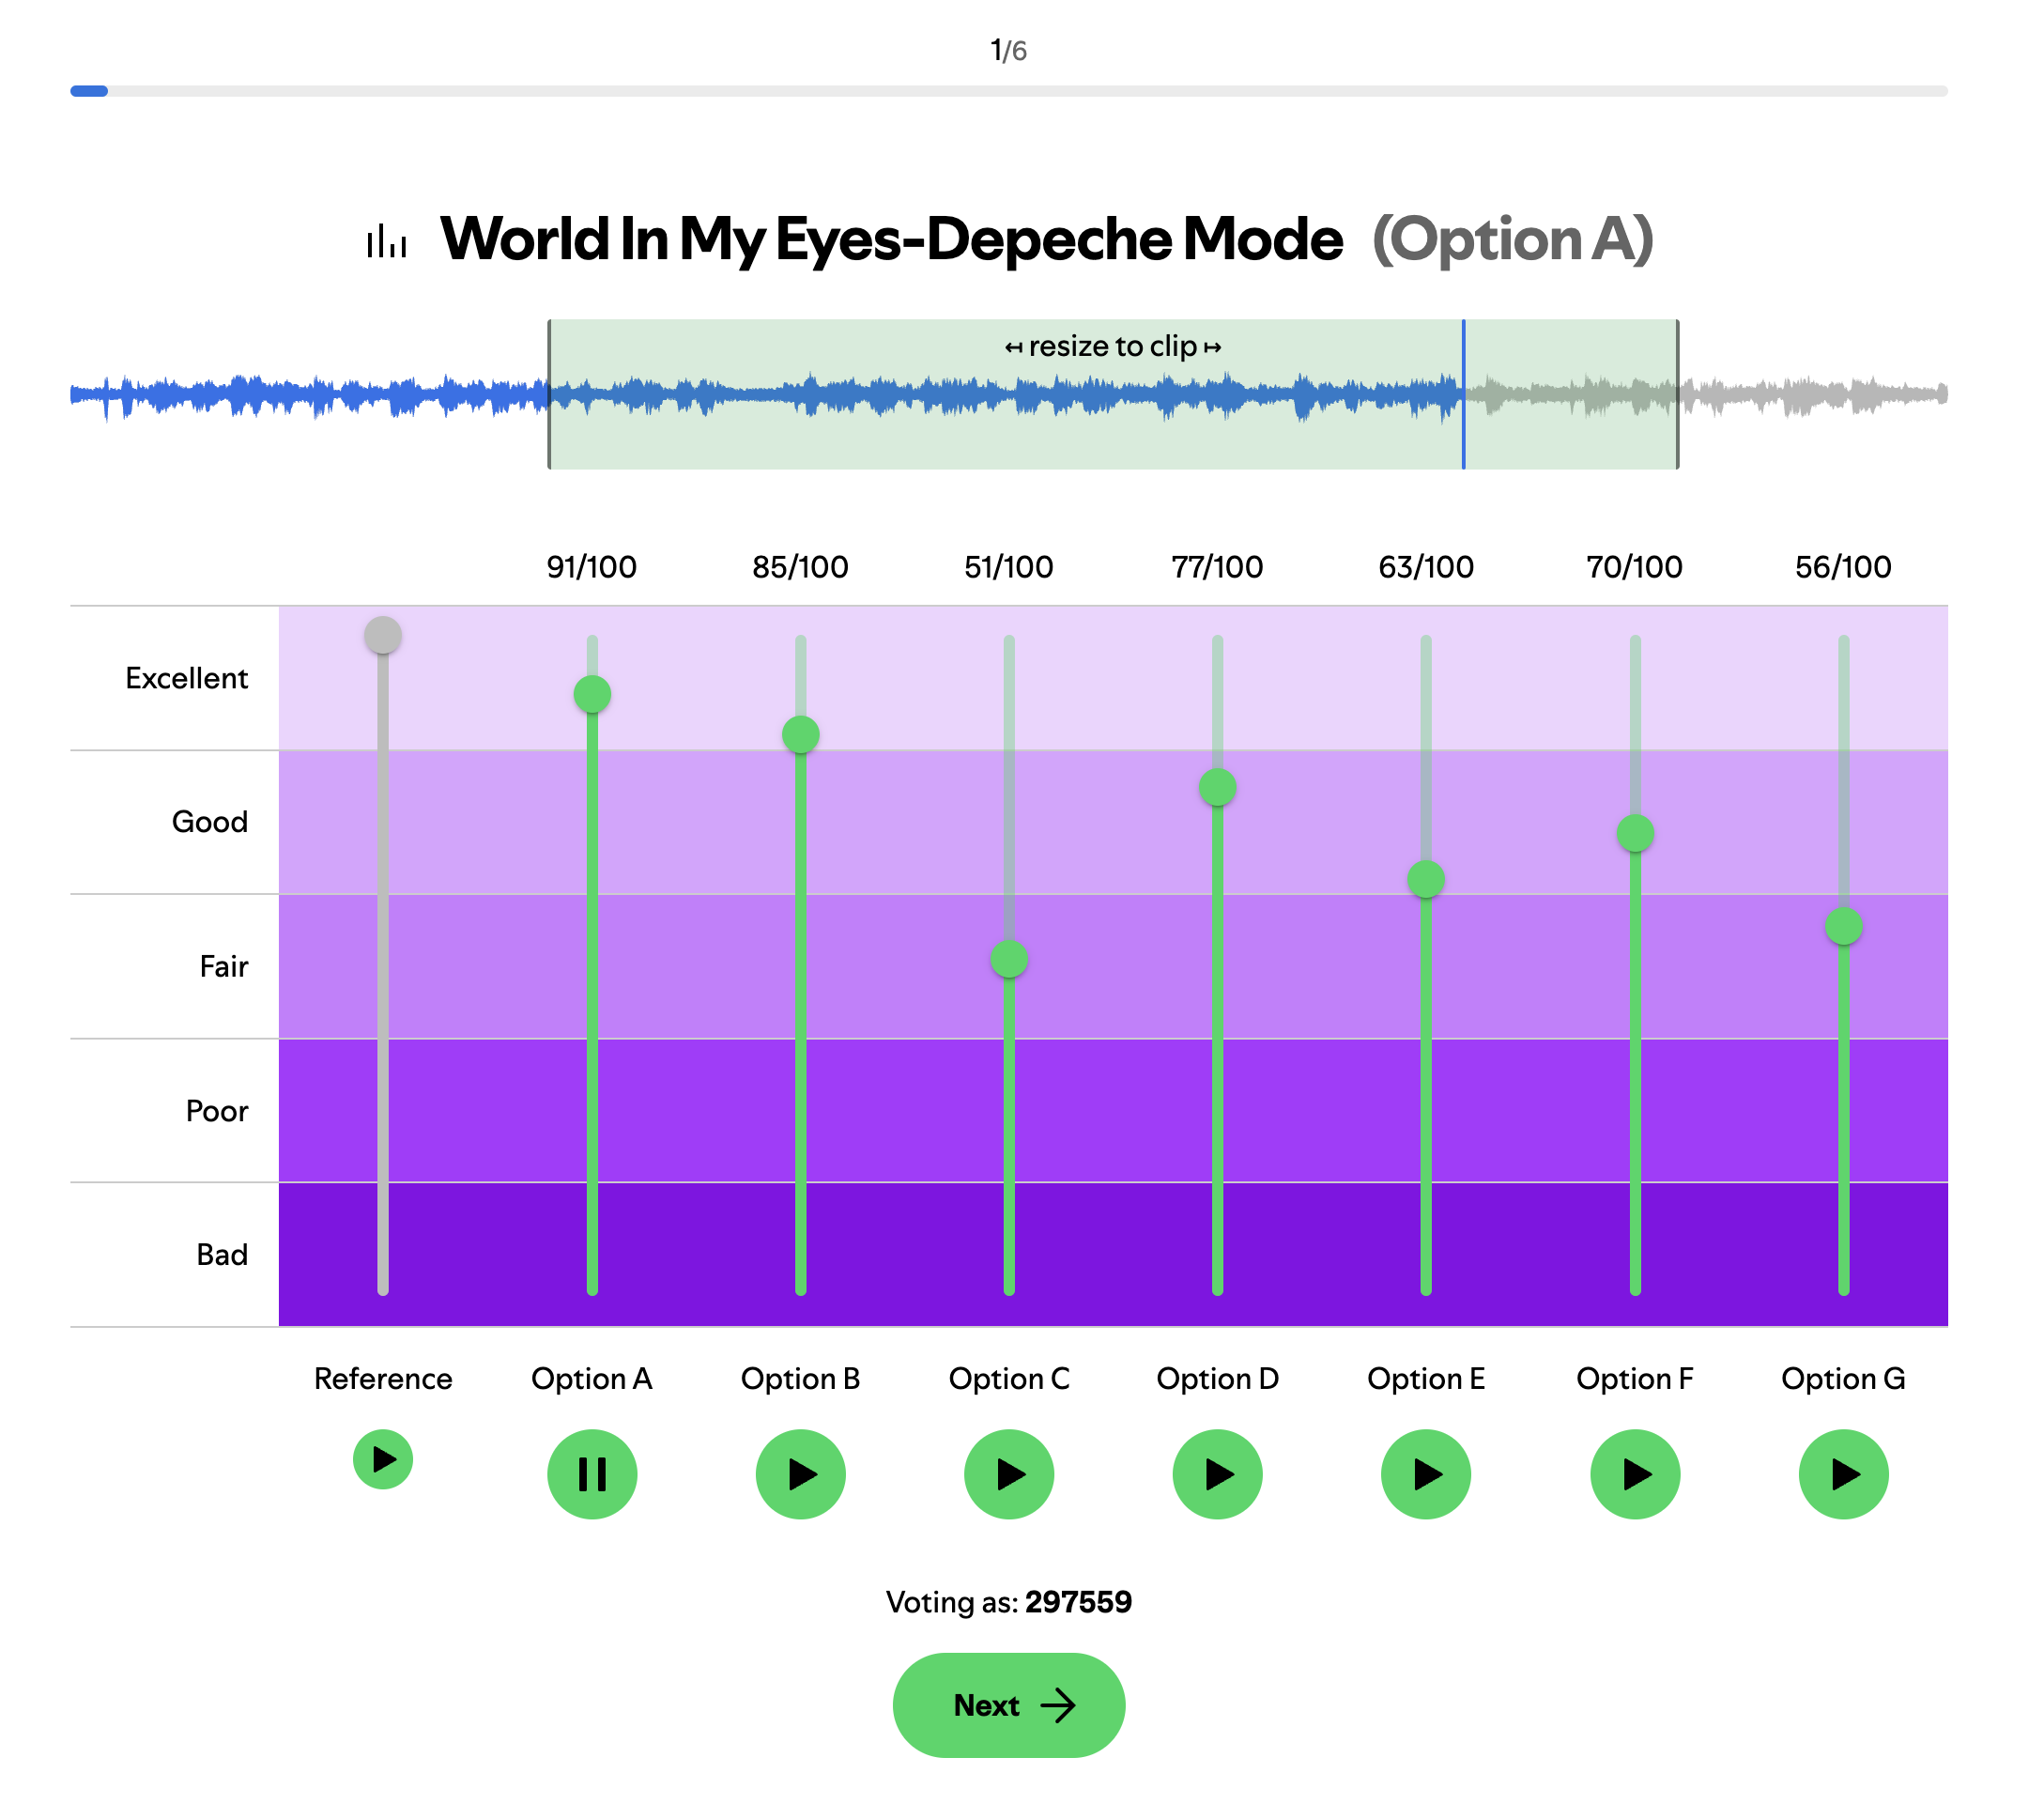
\includegraphics[width=0.65\textwidth]{screenshot_cropped.png}}
\vspace{-0.7cm}
\caption{The experiment interface used in the perceptual evaluation.}
\label{fig:interface}
\end{figure*}

\subsection{Participants}

A subjective test was conducted with 29 participants, comprising 22 males, six females, and one participant who preferred not to disclose their gender. Age data were available for 28 participants, ranging from 20 to 60 years, with a mean age of 36.6 years and a standard deviation of 10.0. Generally, participants who were over 18 years of age and had no hearing impairment were invited to participate in the study. Before participating, they received an information letter with detailed instructions on the experiment. In the laboratory, the participants were always accompanied by a researcher conducting the study. If necessary, further details were explained to them upon their arrival at the laboratory. 

During the experiment, the participant would listen to audio on commercial headphones. No risk was foreseen to the participant, and they were informed in advance that the experiment could be terminated at any point without giving a justification. If they volunteered to participate, they signed a consent form that was kept separate from any data collected through rankings and questionnaires. There was no reward for participating in the experiment. After informed consent, demographic information and experience with streaming services were collected using a questionnaire with a randomized identification number. 

\subsection{Audio Stimuli}
\label{subsec:audio_stimuli}
All audio stimuli consisted of a commercially recorded music track combined with a speech recording. The speech recordings were generated using a commercial \gls{tts} service, with the text being extracted from the Wikipedia\footnote{\url{https://en.wikipedia.org/}} page of the track's primary artist. To balance the gender of the speech voice, 50\% of the tracks were assigned a male \gls{tts} voice and 50\% a female \gls{tts} voice. The mono speech recording with no music was used as the reference signal for each track. Full details can be found in \cref{app:tracks}.

Each variant of a track was created by applying binaural panning of the speech signal at angles \{45L, 30L, 15L, 0, 15R, 30R, 45R\} (where L and R denote left and right, and the number denotes the panning azimuth in degrees from the centre line), as shown in \cref{fig:binauralPanning}. Binaural panning was achieved by convolving the mono speech signal with the left and right \glspl{hrir} recorded by binaural microphones on the KEMAR dummy head subject of the SADIE II database~\cite{armstrongPerceptualEvaluationIndividual2018}. This database of \glspl{hrir} contains a set in which the excitation sound came from the exact angles specified; no interpolation of the \gls{hrir} coefficients was performed. A block diagram for a single azimuth is shown in \cref{fig:stimulusCreation}, in which solid lines represent audio signals, and the dashed line represents duration metadata. The \enquote{Upmix} block represents a simple mono-to-stereo process whereby a mono recording is copied into both the left and right channels. The \enquote{Trim} block represents a process where the music excerpt is truncated to match the length of the binaurally panned speech. The \enquote{Normalize loudness} blocks represent changes in audio gain to ensure that the resulting loudnesses of both speech and music were equal.

\begin{figure}[hbt]
\centering
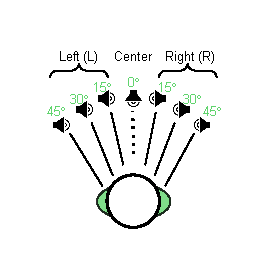
\includegraphics[trim=0.6cm 0.7cm 0.6cm 0.6cm, clip=true,width=0.68\columnwidth]{speech_angles.pdf}
\caption{The binaural panning of the speech signal at the different angles.}
\label{fig:binauralPanning}
\end{figure}

\begin{figure}[!hbtp]
\centering
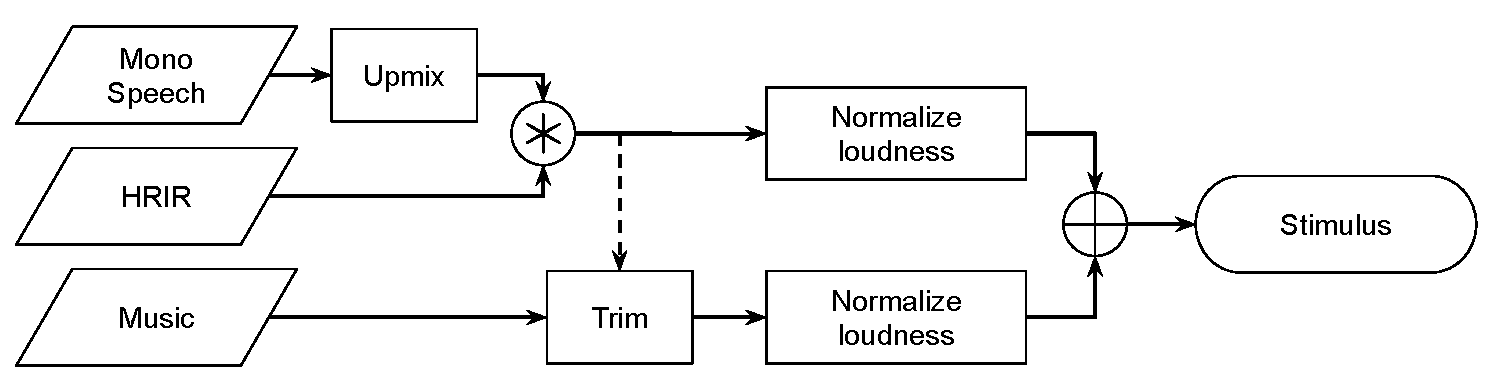
\includegraphics[width=\columnwidth]{binaural_stimulus_creation_thick_lines.pdf}
\caption{Block diagram of the audio stimulus creation process for a single azimuth. Solid lines represent audio signals, the dashed line represents duration metadata, the $\ast$ operator represents channel-wise convolution, and the $+$ operator represents channel-wise addition.}
\label{fig:stimulusCreation}
\end{figure}

Once the binaurally panned speech signal was created, an excerpt of the music track was selected to be (1) musically representative of the track as a whole and (2) precisely the same length as the speech signal. The method of finding a representative section is detailed in~\cite{jehanExtractingExcerptMedia2018}. The speech and music signals were then normalized to the same loudness using the pyloudnorm library~\cite{steinmetzPyloudnormSimpleFlexible2021} (which is an implementation of the ITU-R BS.1770 standard~\cite{itu-r-bs.1770-4AlgorithmsMeasureAudio2015}) and summed to produce the final audio stimuli. In total, six different music tracks were selected, each combined with a different speech recording. The speech recordings were generated using both male and female voices, with three recordings featuring male voices and three featuring female voices. Full details are given in \cref{app:tracks}.

\subsection{Procedure and Experiment Interface}
In the experiment, participants could first adjust the volume to a comfortable level for themselves~\cite{itu-r-bs.1534-3MethodSubjectiveAssessment2023}. The application then presented the interface shown in \cref{fig:interface} to familiarize them with the experimental procedures and the different equipment. This was done before the formal experiment, which involved listening to and rating various audio clips. Each session lasted up to 30 minutes.

Before the start of the experiment, participants were asked four questions: (1) How old are you?, (2) What is your gender? (Male/Female/Other/Prefer not to say), (3) How often do you use streaming services to listen to the following? Music streaming (A. Never use/B. Daily/C. Weekly/D. Monthly), How many hours do you listen to B/C/D?, Podcast (A. Never use/B. Daily/C. Weekly/D. Monthly), How many hours do you listen to B/C/D?, and (4) Do you consider yourself an expert listener? (A. Yes/B. No/C. I do not know).

Participants are presented with a reference signal along with the seven variants described in \cref{subsec:audio_stimuli}, and are asked to rate each based on how pleasant it is to listen to compared to the reference. The ranking scale follows the \gls{mushra} standard in that the opinion is a numeric value between 0 and 100, with the scale split into five equal sections marked by the words \enquote{Excellent}, \enquote{Good}, \enquote{Fair}, \enquote{Poor}, and \enquote{Bad}. Both the order of the variants and the order of the tracks are randomized for each subject, and the names of the variants are replaced with anonymized versions (see \cref{fig:interface}). The test procedure differs from \gls{mushra} in that the variants for each track do not contain a hidden reference or hidden anchor. This is because the subjects were not asked to evaluate a signal degradation but rather a new signal assumed to be more pleasant than the reference. The information collected by the test interface comprised the ratings given to each variant.

After the experiment, participants were asked to complete a questionnaire about their listening experience. In particular, they were asked:
\begin{enumerate*}
    \item Can you justify what influenced your ranking of spatialized voice in music? (with a free-text answer)
    \item Do you prefer female or male voice in music? (A. Female voice, B. Male voice, C. No difference, or D. I do not know)
    \item What did you think about the relationship between the volume of voice and music? (A. The voice was: too quiet, good, too loud, B. The music was: too quiet, good, too loud).
    \item Do you have any further feedback on the experiment? (with a free-text answer).
\end{enumerate*}

The experiment interface, in \cref{fig:interface}, presented the participant with (for each track) a waveform display depicting the track, the track title, the artist name, a set of vertical sliders to give their rating of each variant, and a play/pause button for each variant in addition to the reference. When audio is playing, it is looped, and the waveform display can be used to set the loop points.


\section{Results and Analysis}
\label{sec:results_analysis}

The test participants were informed that a higher score indicated a greater pleasantness, but were given only basic instructions regarding the exact value of the score. Therefore, in the analysis, we assume that the scores are ordinal but with unequal intervals, and hence we only use statistical tests on the ranks of the scores. Ranks are calculated per-person-per-track. 

\subsection{Comparison of Centre to Non-Centre Preference}
\label{sec:noncentrepref}

In \cref{subsec:audio_stimuli}, it was established that the reference signal was a monophonic speech recording. It is standard practice that, by default, a monophonic audio signal is placed exactly in the centre of a stereo rendering. The perceptual evaluation, therefore, assesses whether the test participants gave any preference to the non-centred variants of panned speech. To do this, a Boolean variable was assigned, denoting whether the top choice was centre or non-centre. If there was a tie, the centre won. This new dataset comprises a list of 174 preferences (29 participants $\times$ 6 tracks).

A ratio $R$ representing the proportion of non-centre preference was calculated by $S/N$ where $S$ is the number of results indicating a non-centre preference and $N$ is the total number of results. Hence, $R$ is in the range $[0,1]$ where $0$ means that the voice overlay was always rated best in the central position, and $1$ means that the voice overlay was always rated best in a non-centre position. These values are presented in \cref{table:ratios}, both for the entire dataset and separated by music track. Under the previously mentioned assumption that the default location is centrally panned, the given values of $R$ can be interpreted as the proportion of instances in which the default option (centre-panned) was suboptimal. As can be seen from the table, across all tests (i.e., the group labelled \enquote{All}) the default position was suboptimal in 59\% of cases.

\begin{table}[h!]
\centering
\caption{Ratios ($R$) of centre to non-centre preference for all test results and each individual track.}
\begin{tabular}{lccccc}
\toprule
Group & $S$ & $N$ & $R$ \\
\midrule
Brown Eyed Girl & 18 & 29 & \num{0.62} \\
Everyday Is A Winding Road & 18 & 29 & \num{0.62} \\
Fake Plastic Trees & 22 & 29 & \num{0.76} \\
Fly Me To The Moon & 16 & 29 & \num{0.55} \\
World In My Eyes & 14 & 29 & \num{0.48} \\
bad guy & 15 & 29 & \num{0.52} \\
All & 103 & 174 & \num{0.59} \\
\bottomrule
\end{tabular}

\label{table:ratios}
\end{table}

To further analyse these results, we used a series of $\chi^2$ tests to assess whether any of the categorical data collected in the questionnaire explained the participants' preferences. \Cref{table:chi2} shows the results of these tests. They show that the only variable that is significantly correlated to non-centre preference is the assessor themselves. Essentially, the participants had preferences as to in which position the voice sounds most pleasant, but the demographic data collected in the survey did not explain those preferences. This matches the conclusion of Torcoli et. al regarding the importance of personalized loudness differences between speech and music  \cite{torcoliPreferredLevelsBackground2019}. Although that study found statistical links between loudness preferences and factors such as assessor age and listening experience, and the audio material itself, conversely, this study did not find such links for the voice panning position. This indicates that the reasons for the participants' preferences remain unknown.

\begin{table}[h!]
\setlength{\tabcolsep}{3pt}
\centering
\caption{Results of $\chi^2$ tests between independent variables and non-centre preference. The column \enquote{CV (DOF)} shows the critical values in the $\chi^2$ distribution for 95\% confidence with the given degrees of freedom. Significant variables are shown in bold.}
\begin{tabular}{lccc}
\toprule
Variable & CV (DOF) & $\chi^2$ & P-value \\
\midrule
\textbf{Participant} & \textbf{41.34 (28)} & \textbf{75.33} & \textbf{\num{3.24e-06}} \\
Gender & 5.99 (2) & 2.82 & 0.24 \\
Expert listener & 5.99 (2) & 2.27 & 0.32 \\
Track & 11.07 (5) & 5.83 & 0.32 \\
Voiceover gender  & 3.84 (1) & 0.86 & 0.35 \\
Age range  & 5.99 (2) & 1.48 & 0.48 \\
Podcast usage  & 7.82 (3) & 2.49 & 0.48 \\
Music streaming usage & 5.99 (2) & 0.31 & 0.86 \\
\bottomrule
\end{tabular}
\label{table:chi2}
\end{table}

\subsection{Comparison of Ranked Azimuths}
\label{sec:comparison_of_ranked_azimuths}

In \cref{sec:noncentrepref} it was established that the central panning position is sometimes suboptimal. In this section, the scores given to individual panning positions are assessed to establish whether any particular position is more desirable. To that end, \cref{average_ranks} shows box plots of the ranks given to each position.

While the confidence intervals of some adjacent panning positions do overlap, there is a clear general trend that the more extreme panning received worse ranks. However, all positions received the full range of the ranks, indicating that there was clear disagreement between the test participants. This aligns with the observation from \cref{sec:noncentrepref} that the participants' choices were highly personal.

\begin{figure}[h]
\centering
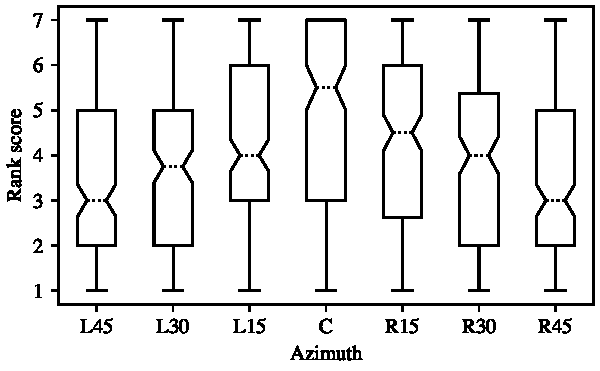
\includegraphics[width=\columnwidth]{rank_boxplots.pdf}
\caption{Box plots of panning position ranks across all tracks. Dotted lines show the median and notches show the 95\% confidence interval calculated with Gaussian-based asymptotic approximation \cite{mcgillVariationsBoxPlots1978}.}
\label{average_ranks}
\end{figure}

To test for statistically significant differences between azimuths, a Kruskal-Wallis-H test is first conducted with the null hypothesis that all azimuths are ranked equally. With a confidence value of 95\% and seven azimuth classes, a critical value of $12.59$ is found in the $\chi^2$ distribution with six degrees of freedom. The result of the test is an H-statistic of 18.0 with a p-value of 0.00636. Therefore, the null hypothesis is rejected and it can be concluded that at least one of the azimuths is ranked differently from the others. To determine which one, a Dunn's post-hoc test with Bonferroni correction is performed to compare pairwise p-values. The results of all pairs that included \enquote{Centre} are shown in \cref{table:posthoc}. All other pairs had p-values of 1 and are omitted from the table. There are two azimuths with a significant difference from \enquote{Centre} - \enquote{Left 45} and \enquote{Right 45}. Looking at the median scores of these two classes, it can be concluded that the extreme-panned speech was indeed less highly rated than the more modest panned or centred speech. Interestingly, even though there are no other statistically significant differences, the \textit{confidence} of a difference from \enquote{Centre} is lower on the right side. We speculate that this might be due to the \enquote{right-ear advantage} -- a phenomenon in which a person is more easily able to interpret a voice presented to the right ear than the left~\cite{tanakaNeurophysiologicalEvaluationRightEar2021}. More data would need to be collected to test this speculation.

Similar Kruskal-Wallis-H tests were performed with data for single tracks, but the null hypothesis could not be rejected for any of them.

\begin{table}[htb]
\caption{Medians and p-values for pairwise differences between the centre-panned voice and all other azimuths. Significant differences are shown in bold. Centre median value is shown for comparison.}
\setlength{\tabcolsep}{2.5pt}
\centering
\begin{tabular}{lccccccc}
\toprule
 & \textbf{L45} & L30 & L15 & \textcolor{gray}{C} & R15 & R30 & \textbf{R45} \\
\midrule
Median & \textbf{53.0} & 54.5 & 55.0 & \textcolor{gray}{63.0} & 59.0 & 57.0 & \textbf{55.0} \\
P-value & \textbf{0.006} & 0.064 & 0.341 & - & 1.000 & 0.267 & \textbf{0.015} \\
\bottomrule
\end{tabular}

\label{table:posthoc}
\end{table}


\subsection{Analysis of Free-Text Responses}
To reiterate, the questions with free-text responses given to test participants were \enquote{Can you justify what influenced your ranking of spatialized voice in music?} and \enquote{Do you have any further feedback on the experiment?}. The participants answered both questions with similar information and therefore the responses were combined. Subsequently, they were thematically analysed and classified by the authors. The themes mentioned are shown in \cref{table:freetextthemes} alongside the number and percentage of participants who mentioned them.

The most prominent overarching theme was that difficulty in hearing the panned speech or its lack of clarity was the primary factor in the participants' ratings of pleasantness. Some participants provided more detailed feedback, specifying that the music was too loud or that the type of music affected their scores. Eight participants stated that they felt the voice was always clearer on either the left or the right, and seven stated that they always wanted the voice to be in the centre. Smaller sets of participants mentioned that clashes between any singing voice in the music and the speech led to lower ratings. They also noted that the pitch of the voice affected their ratings, either positively or negatively, depending on the music. A similarly small group mentioned that the spatial factors affected their scores. Some comments also specifically mentioned that speech with more extreme panning was less pleasant, which is also reflected in the data (see \cref{sec:comparison_of_ranked_azimuths}).

\begin{table}[h]
    \centering
    \caption{Counts of test participants who mentioned that specific factors affected their ratings.}
    \begin{tabular}{lcc}
        \toprule
        Theme & Count & Percentage \\
        \midrule
        Clarity of voice / listening effort & 17 & 59\% \\
        Music too loud & 10 & 34\% \\
        Left/right preference & 8 & 28 \% \\
        Centre preference & 7 & 24\% \\
        Clash between singing and speech & 5 & 17\% \\
        Speech pitch & 5 & 17\% \\
        Speech location / spatial factors & 4 & 14\% \\
        Music type / genre & 4 & 14\% \\
        \bottomrule
    \end{tabular}
    \label{table:freetextthemes}
\end{table}

Based on these findings, it is suggested that further experiments stratify the music tracks into those with and without strong vocals, include a more varied range of music genres, and apply less extreme panning to the voiceover.

\subsection{Analysis of Loudness Perception}
\label{sec:loudness_perception}

Recall that participants were asked if the music and voice were too loud, too quiet, or good. A tabulation of their responses can be found in \cref{tab:loudness}. The raw results are skewed towards the music being too loud or good, and the voice being good or too quiet. Bearing in mind that, in actuality, both were normalized to equal loudness, it can be speculated that participants considered the music to be an interfering sound source and the voice to be the desired sound source. This was contrary to the original assumptions of the authors and needs to be considered in future iterations of the experiment. It does, however, mirror the findings of the free-text responses - voice clarity was paramount.

\begin{table}[h]
    \centering
    \caption{Test participants' opinions of the loudness of music and voice.}
    \begin{tabular}{lcc}
        \toprule
            & Voice & Music \\
        \midrule
        Too loud & 2 & 18 \\
        Good & 18 & 10 \\
        Too quiet & 9 & 1 \\
    \bottomrule
    \end{tabular}
    \label{tab:loudness}
\end{table}

\subsection{Discussion}
\label{sec:discussion}
A constant source of uncertainty during data analysis was the relatively small number of both tracks and participants. In particular, only six tracks were used to limit the duration of each test session. In reality, it was not enough to draw strong statistical conclusions about differences between tracks. 

Furthermore, several of the statistical tests used are based on the assumption that all data are independent. It could be argued that the data collected are not strictly independent since each participant scored multiple tracks. This was a practical compromise made to gather enough data for any analysis. It is a known problem that subjective tests of this variety are slow and costly, and recent efforts in crowdsourcing \gls{mushra} tests have proven fruitful~\cite{lechlerCrowdsourcingMUSHRATests2025} (although this work focused on assessing solo speech signals rather than music).

\section{Conclusions and Future Work}
\label{sec:conclusions}
A perceptual evaluation was performed to determine the pleasantness of music mixed with voice that has been binaurally panned to various angles by convolving the signal with an \gls{hrir}. Participants were presented with a \gls{mushra}-like test in which they moved sliders to give their opinions of the different panning azimuths. The raw scores were transformed into ranks on a per-person-per-track basis.

The non-centre positions were preferred over the centre in 59\% of the test cases, and the ratings given by test participants were highly personal. However, the demographic data collected about the participants did not explain their choices.

Kruskal-Wallis tests revealed that the outermost azimuths were consistently ranked lower than the moderately panned and centre azimuths. There was also the implication that the voice panned to the right was ranked higher than that on the left, but as stated above, more data would be required for confirmation.

The free-text explanations given by the participants showed that \enquote{listening effort} or \enquote{voice clarity} were the factors that influenced the pleasantness of the audio for the highest number of people. They suggest that to increase overall pleasantness, a voiceover should be cleanly separated from any vocals in the music, although the best method of separation remains unclear. Alongside this, there were indications that other factors relating to listeners' personal preference should be investigated in future experiments.

Based on these findings, we suggest that further experiments be performed in which more tracks and more test participants are used. The musical excerpts chosen should be controlled so that they have either strong vocals or a lack thereof throughout, and the vocal overlays should be panned more towards the centre and in finer increments.

\section{Acknowledgements}
This study was supported by the Knowledge Foundation, Sweden, through the Human-Centered Intelligent Realities (HINTS) Profile Project (20220068), and the Information Retrieval in Embedded Systems for Audiovisual Artistic Processes (IRESAP) project (20220037).

\bibliography{svim.bib}
\bibliographystyle{jaes.bst}

\clearpage

\appendix
\onecolumn

\section{\MakeUppercase{Details of audio stimuli}}
\label{app:tracks}

The audio stimuli contain copyrighted material and therefore cannot be distributed. For reproducibility, the parameters to recreate them are provided in this appendix.

\subsection*{Track metadata}

\begin{table*}[h]
% \scriptsize
\centering
\begin{tabular}{llrrl}
\toprule
Title & Artist & Start Time & Duration & Voiceover Gender \\
\midrule
Everyday Is A Winding Road & Sheryl Crow & 136.19 & 21.04 & male \\
Fly Me To The Moon & Frank Sinatra & 64.00 & 20.06 & male \\
Fake Plastic Trees & Radiohead & 173.32 & 23.37 & female \\
Brown Eyed Girl & Van Morrison & 81.08 & 19.88 & female \\
bad guy & Billie Eilish & 114.67 & 16.77 & female \\
World In My Eyes & Depeche Mode & 169.49 & 13.84 & male \\
\bottomrule
\end{tabular}
\end{table*}


\subsection*{Voiceover text}

\noindent\textbf{Sheryl Crow}\\Sheryl Suzanne Crow (born February 11, 1962) is an American singer, musician, songwriter, and actress. She is noted for her optimistic and idealistic subject matter, and incorporation of genres including rock, pop, country, folk, and blues. She has released twelve studio albums, five compilations, and three live albums, and contributed to several film soundtracks.
\\\\
\noindent\textbf{Frank Sinatra}\\Francis Albert Sinatra (born December 12, 1915) was an American singer and actor. Nicknamed the "Chairman of the Board" and "Ol' Blue Eyes", he is regarded as one of the most popular entertainers of the 20th century. Sinatra is among the world's best-selling music artists, with an estimated 150 million record sales globally.
\\\\
\noindent\textbf{Radiohead}\\Radiohead are an English rock band formed in Abingdon, Oxfordshire, in 1985. They comprise Thom Yorke; brothers Jonny Greenwood and Colin Greenwood; Ed O'Brien; and Philip Selway. They have worked with the producer Nigel Godrich and the cover artist Stanley Donwood since 1994. Radiohead's experimental approach is credited with advancing the sound of alternative rock.
\\\\
\noindent\textbf{Van Morrison}\\Sir George Ivan "Van" Morrison OBE (born 31 August 1945) is a Northern Irish singer-songwriter and musician whose recording career started in the 1960s. Morrison's albums have performed well in the UK and Ireland, with more than 40 reaching the UK top 40, as well as internationally, including in Germany, the Netherlands and Switzerland.
\\\\
\noindent\textbf{Billie Eilish}\\Billie Eilish Pirate Baird O'Connell (born December 18, 2001) is an American singer-songwriter. She first gained public attention in 2015 with her debut single "Ocean Eyes", written and produced by her brother Finneas O'Connell, with whom she collaborates on music and live shows.
\\\\
\noindent\textbf{Depeche Mode}\\Depeche Mode are an English electronic music band formed in Basildon, Essex in 1980. Originally formed with the lineup of Dave Gahan, Martin Gore, Andy Fletcher and Vince Clarke, the band currently consists of Gahan and Gore.
\\\\

\twocolumn

\clearpage % include as there are formatting conflicts with the end of the manuscript in 2-column format and the Biography section. This will be rectified in the final page layout by the journal. 

%Biography
\biography{Richard Mitic}{richard.jpg}{Richard Mitic is a doctoral candidate at Mälardalen University, currently researching spatial audio, digital signal processing, and large-scale music information retrieval. He holds a masters degree in Music and Electronics from the University of Glasgow where he specialised in digital electronics and audio processing. He has 14 years experience in industry, starting as a researcher of media streaming protocols and participating in \glsxtrshort{mpeg} standardization, later progressing into the music industry where he wrote software for music streaming, media transcoding, real-time audio, and embedded devices. }
 
\biography{Majed Elwardy}{majed.png}{Majed Elwardy is a Lecturer in Computer Science at \gls{bth}, Sweden. He received his Ph.D. in Computer Science from \gls{bth} in 2025, where his research focused on 360-degree video quality assessment and user behavior in virtual reality. His research lies at the intersection of human–computer interaction and immersive technologies, with particular interests in immersive multimedia, quality of experience, signal processing, user experience evaluation, cybersickness, and pedagogy-driven approaches for \gls{xr} education.}

\biography{Veronica Sundstedt}{veronica.jpg}{Veronica Sundstedt is a Professor in Computer Science at \gls{bth}, bringing extensive international experience gained at institutions including Trinity College Dublin, the University of Bristol, and the University of Bath. She holds a Ph.D. in Computer Graphics from the University of Bristol. Her research expertise lies in the intersection of computer graphics and perception, focusing particularly on perceptually-based rendering, novel interaction techniques, and eye tracking. Her academic contributions include organizing conferences and serving on multiple \glsxtrshort{acm} editorial boards. Currently, she develops and teaches specialized courses at \gls{bth}, and she is the project leader for a new research initiative focused on \enquote{Human-Centered Intelligent Realities (HINTS), funded externally from the Knowledge Foundation (20220068).}}

\biography{Andreas Rossholm}{andreas.jpg}{Andreas Rossholm is a Staff Research Scientist at Spotify where his focus is to secure the perceived audio and video quality from injection to consumption. He received his Ph.D. in Applied Signal Processing from \gls{bth} and has over 15 years experience of both real time and streaming media. Earlier Andreas has worked at Microsoft Skype Division, and before that he worked at Ericsson Mobile Platform as Video Specialist and Manager for Audio and Video R\&D teams.}

\biography{Yan Hu}{yan.png}{Yan Hu is an Associate Professor in the Department of Computer Science at \gls{bth}, Sweden, where she leads the Game and Interactive Systems team. She received her Ph.D. in Computer Science from \gls{bth} in 2017 and began her \gls{xr} research during her postdoctoral studies. Her research interests include human-computer interaction, \gls{xr} interaction, social \gls{xr}, and biometric research in behavior and interaction.}

\end{document}
